\documentclass[aspectratio=169]{beamer}
% Shared Beamer style for this repository.
\usepackage[fontset=none]{ctex}
\usepackage{fontspec}
\setmainfont{DejaVu Serif}
\setsansfont{DejaVu Sans}
\setmonofont{DejaVu Sans Mono}
\setCJKmainfont{Noto Serif CJK SC}[BoldFont={Noto Serif CJK SC Bold}]
\setCJKsansfont{Noto Sans CJK SC}[BoldFont={Noto Sans CJK SC Bold}]
\setCJKmonofont{Noto Sans Mono CJK SC}

\usetheme{Madrid}
\usefonttheme{serif}
\setbeamertemplate{navigation symbols}{}
\setbeamertemplate{footline}[frame number]

\usepackage{graphicx}
\usepackage{amsmath,amssymb}
\usepackage{booktabs}
\usepackage{array}
\usepackage{xcolor}
\usepackage{listings}
\usepackage{tikz}
\usetikzlibrary{shapes,arrows,positioning}

% Color system
\definecolor{dcPrimary}{RGB}{21,101,117}
\definecolor{dcSecondary}{RGB}{140,115,72}
\definecolor{dcAccent}{RGB}{184,92,63}
\definecolor{dcMuted}{RGB}{230,250,252}
\definecolor{dcWarmBG}{RGB}{255,245,230}
\definecolor{dcCodeBG}{RGB}{247,248,250}
\definecolor{dcCodeFrame}{RGB}{200,210,215}

\setbeamercolor{structure}{fg=dcPrimary}
\setbeamercolor{palette primary}{fg=dcPrimary,bg=dcMuted}
\setbeamercolor{palette secondary}{fg=dcSecondary,bg=dcMuted!90}
\setbeamercolor{palette tertiary}{fg=dcPrimary,bg=dcMuted!80}
\setbeamercolor{frametitle}{fg=white,bg=dcPrimary}
\setbeamercolor{title}{fg=dcPrimary}
\setbeamercolor{alerted text}{fg=dcAccent}
\setbeamercolor{item}{fg=dcPrimary}
\setbeamercolor{subitem}{fg=dcSecondary}
\setbeamercolor{block title}{fg=white,bg=dcPrimary}
\setbeamercolor{block body}{bg=dcMuted}
\setbeamercolor{block title example}{fg=white,bg=dcSecondary}
\setbeamercolor{block body example}{bg=dcWarmBG}
\setbeamercolor{block title alerted}{fg=white,bg=dcAccent}
\setbeamercolor{block body alerted}{bg=dcWarmBG}
\setbeamercolor{footline}{fg=dcPrimary}

\lstset{
  basicstyle=\ttfamily\footnotesize,
  backgroundcolor=\color{dcCodeBG},
  frame=single,
  rulecolor=\color{dcCodeFrame},
  numbers=none,
  breaklines=true,
  showstringspaces=false,
  tabsize=2
}


\title{EDA工具与FPGA实践基础}
\subtitle{第二章：开发环境、Linux命令行与首个验证闭环}
\author{Digital Circuit Getting Started}
\date{\today}

\graphicspath{{figures/}}

\begin{document}

% ============ Frame 1: 标题 ============
\begin{frame}
  \titlepage
\end{frame}

% ============ Frame 2: 学习目标 ============
\begin{frame}{学习目标}
\begin{itemize}
  \item 搭建一套开源数字设计工具链（Icarus + GTKWave + Yosys）
  \item 在Linux终端中导航、组织项目目录、执行脚本
  \item 运行仿真、观察波形、理解信号值语义（0/1/X/Z）
  \item 将RTL综合为门级网表，并对比行为与结构的差异
  \item 建立FPGA作为``可重配置硬件沙盘''的直觉
\end{itemize}
\end{frame}

% ============ Frame 3: 全章路线图 ============
\begin{frame}{全章路线图}
\begin{enumerate}
  \item 为什么先跑工具？——即时反馈的认知杠杆
  \item Linux基础与工程目录结构
  \item 仿真流水线：Icarus $\rightarrow$ VVP $\rightarrow$ GTKWave
  \item 读懂波形：时间轴、边沿、X/Z
  \item 综合：RTL 如何变成门级网表
  \item 行为 vs. 结构：仿真与综合之间的语义裂隙
  \item 工具版图：开源、商业与FPGA厂商
  \item FPGA直觉：LUT + 触发器 + 可编程互连
  \item 完整走通：从RTL到比特流
\end{enumerate}
\end{frame}

% ============ Frame 4: 为什么先跑工具？ ============
\begin{frame}{\S1 为什么先把工具跑通？}
\begin{columns}
\column{0.55\textwidth}
\textbf{认知层面的理由：}
\begin{itemize}
  \item 即时反馈是 \alert{认知杠杆}
  \item 写几行RTL $\rightarrow$ 几秒后看到波形变化
  \item 不必先背两章门电路理论再去碰工具
\end{itemize}
\column{0.4\textwidth}
\begin{block}{教学契约}
\small
本章：\textbf{跑通、观察、比对}\\
后续章节：\textbf{设计、优化、解释原理}
\end{block}
\end{columns}
\vspace{0.5em}
\centering
\textit{类比：先学会点火、挂挡、看仪表盘把车开起来，\\再研究发动机怎么转。}
\end{frame}

% ============ Frame 5: GUI vs 命令行 ============
\begin{frame}{\S2 Linux基础：图形界面 vs. 命令行}
\begin{columns}
\column{0.48\textwidth}
\textbf{图形界面}
\begin{itemize}
  \item 点击、拖拽、双击
  \item 上手容易
  \item 难以复现
  \item 无法脚本化
\end{itemize}
\column{0.48\textwidth}
\textbf{命令行}
\begin{itemize}
  \item 输入、执行、观察
  \item 初期门槛稍高
  \item \alert{完全可复现}
  \item \alert{完全可脚本化}
\end{itemize}
\end{columns}
\vspace{0.8em}
\centering
\textbf{数字设计流程天然包含大量重复动作。}\\
命令行赢在稳定性和自动化。
\end{frame}

% ============ Frame 6: 目录结构 ============
\begin{frame}[fragile]{\S2 工程目录结构}
\begin{columns}
\column{0.45\textwidth}
\textbf{标准布局：}
\begin{verbatim}
lab1-breathing-led/
├── rtl/          # HDL源码
├── tb/           # 测试平台
├── sim/          # 仿真脚本与产物
├── synth/        # 综合脚本与结果
├── fpga/         # 板级约束
└── README.md
\end{verbatim}
\column{0.5\textwidth}
\textbf{核心原则：}\\
\textit{源码、测试和生成产物必须分开放。}\\[1em]
\begin{alertblock}{路径直觉}
\texttt{bash sim/run.sh} 在此目录能跑，\\在 \texttt{synth/} 里就跑不通。
\end{alertblock}
\end{columns}
\end{frame}

% ============ Frame 7: 常见坑 ============
\begin{frame}{\S2 高频陷阱}
\begin{columns}
\column{0.48\textwidth}
\begin{alertblock}{Ctrl+C}
在终端里：\textbf{终止}当前进程。\\
复制粘贴用 \texttt{Ctrl+Shift+C} / \texttt{Ctrl+Shift+V}
\end{alertblock}
\column{0.48\textwidth}
\begin{alertblock}{命令找不到}
\begin{itemize}
  \item 先检查：\texttt{which iverilog}
  \item 若为空：\texttt{sudo apt install iverilog}
  \item 安装前务必 \texttt{sudo apt update}
\end{itemize}
\end{alertblock}
\end{columns}
\vspace{0.5em}
\centering
\textbf{黄金法则：}每个工具必须回答三个问题——\\
它输入什么？输出什么？在流程的哪个位置？
\end{frame}

% ============ Frame 8: 仿真流水线 ============
\begin{frame}{\S3 仿真三件套}
\centering
\textbf{三个工具，一条数据流：}
\vspace{0.5em}

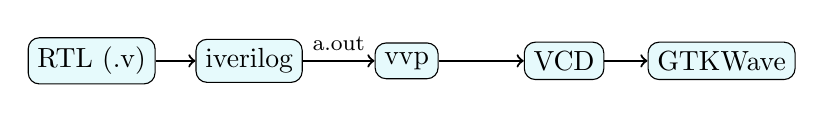
\begin{tikzpicture}[node distance=2cm, auto]
  \node[draw, rounded corners, fill=dcMuted] (rtl) {RTL (.v)};
  \node[draw, rounded corners, fill=dcMuted, right of=rtl] (iv) {iverilog};
  \node[draw, rounded corners, fill=dcMuted, right of=iv] (vvp) {vvp};
  \node[draw, rounded corners, fill=dcMuted, right of=vvp] (vcd) {VCD};
  \node[draw, rounded corners, fill=dcMuted, right of=vcd] (gtkw) {GTKWave};
  \draw[->, thick] (rtl) -- (iv);
  \draw[->, thick] (iv) -- node[above] {\footnotesize a.out} (vvp);
  \draw[->, thick] (vvp) -- (vcd);
  \draw[->, thick] (vcd) -- (gtkw);
\end{tikzpicture}

\vspace{1em}
\begin{tabular}{lll}
\toprule
\textbf{工具} & \textbf{作用} & \textbf{产物} \\
\midrule
Icarus & 编译RTL+TB & 可执行文件 (a.out) \\
VVP & 执行仿真 & 波形文件 (.vcd) \\
GTKWave & 可视化 & 屏幕显示 \\
\bottomrule
\end{tabular}
\end{frame}

% ============ Frame 9: 三步得波形 ============
\begin{frame}{\S3 三步得到波形}
\begin{block}{第一步：编译}
\texttt{iverilog -o sim/tb.vvp rtl/breathing\_led.v tb/tb\_breathing\_led.v}
\end{block}
\begin{block}{第二步：运行}
\texttt{vvp sim/tb.vvp}
\end{block}
\begin{block}{第三步：查看}
\texttt{gtkwave sim/tb.vcd}
\end{block}
\vspace{0.5em}
\centering
\textit{三步都成功，你就闭环了第一个验证回路。}
\end{frame}

% ============ Frame 10: 信号值 ============
\begin{frame}[fragile]{\S4 波形中的四种信号值}
\textbf{数字仿真中的四种取值：}
\vspace{0.5em}

\begin{tabular}{clcl}
\toprule
\textbf{值} & \textbf{含义} & \textbf{何时出现} & \textbf{严重程度} \\
\midrule
\texttt{0} & 逻辑低 & 正常运行 & --- \\
\texttt{1} & 逻辑高 & 正常运行 & --- \\
\texttt{X} & 未知 & 未初始化、仿真初始阶段、多驱动冲突 & \alert{需警惕} \\
\texttt{Z} & 高阻态 & 三态、未驱动 & \alert{需检查} \\
\bottomrule
\end{tabular}

\vspace{0.8em}
\textbf{Testbench中的时钟生成：}
\begin{verbatim}
always #5 clk = ~clk;    // 周期 = 10 个时间单位
\end{verbatim}
\end{frame}

% ============ Frame 11: 边沿与采样 ============
\begin{frame}{\S4 时钟边沿与寄存器采样}
\begin{columns}
\column{0.55\textwidth}
\textbf{组合逻辑：}
\begin{itemize}
  \item 输入稳定后输出才变化
  \item 延迟称为 \textit{传播延迟}
\end{itemize}

\textbf{时序逻辑：}
\begin{itemize}
  \item 寄存器在 \texttt{posedge clk} 采样
  \item 输出在边沿 \textit{之后} 更新
  \item 必须在下一个边沿前稳定（建立时间）
\end{itemize}
\column{0.4\textwidth}
\begin{block}{视觉检查}
在GTKWave中：\\
$\bullet$ 放大到单时钟周期\\
$\bullet$ 确认数据在上升沿后变化\\
$\bullet$ 复位后不应残留X
\end{block}
\end{columns}
\end{frame}

% ============ Frame 12: 呼吸灯波形 ============
\begin{frame}{\S4 呼吸灯波形示例}
\textbf{在GTKWave中你应该看到：}
\begin{itemize}
  \item \texttt{duty}：三角波，先升后降（仿真中为缩微版参数）
  \item \texttt{pwm\_cnt}：快速锯齿波（仿真中为缩微版参数）
  \item \texttt{pwm\_out}：脉宽调制，窄 $\rightarrow$ 宽 $\rightarrow$ 窄
\end{itemize}

\vspace{0.5em}
\centering
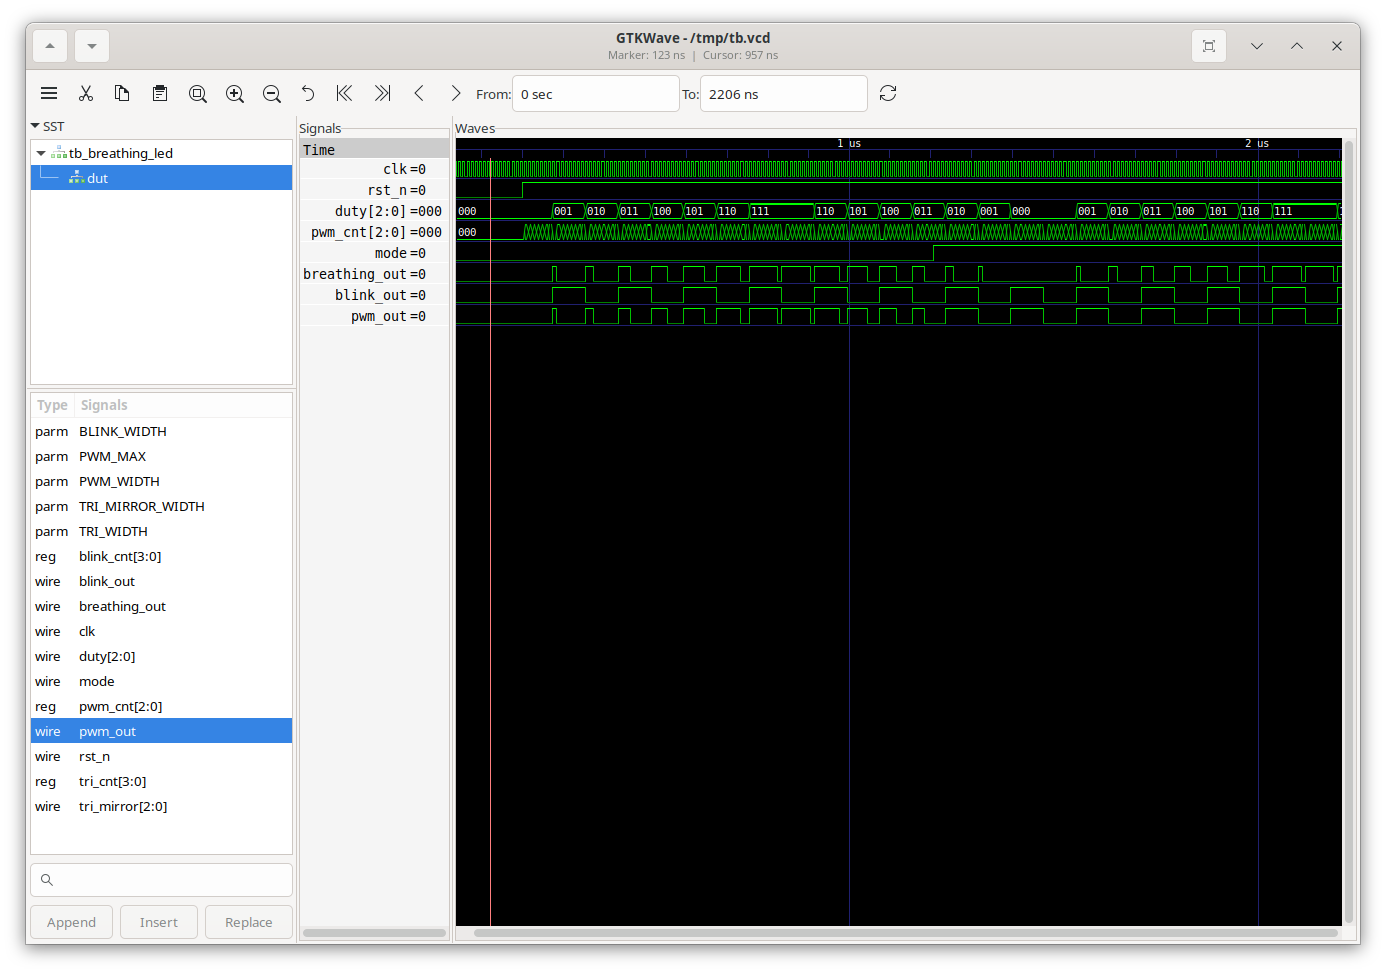
\includegraphics[width=0.85\textwidth]{fig02-gtkwave-screenshot.png}
\end{frame}

% ============ Frame 13: 综合概述 ============
\begin{frame}[fragile]{\S5 综合：RTL $\rightarrow$ 门级网表}
\begin{columns}
\column{0.48\textwidth}
\textbf{综合做什么：}
\begin{enumerate}
  \item 解析RTL（Verilog）
  \item 从 \texttt{always @(posedge clk)} 推断寄存器
  \item 从 \texttt{assign} 推断组合逻辑
  \item 优化：常量传播、死代码消除
  \item 输出通用门单元网表
\end{enumerate}
\column{0.48\textwidth}
\textbf{一条命令：}
\begin{verbatim}
yosys -p "read_verilog rtl/breathing_led.v;
  synth -top breathing_led;
  write_verilog synth/breathing_led_synth.v"
\end{verbatim}
\vspace{0.5em}
\alert{网表的``惊喜''：}你的 \texttt{counter} 变成了几十个 \texttt{\$\_DFF\_P\_} 单元。
\end{columns}
\end{frame}

% ============ Frame 14: 网表长什么样 ============
\begin{frame}[fragile]{\S5 网表长什么样}
\textbf{RTL（人写的）：}
\begin{verbatim}
always @(posedge clk or negedge rst_n)
  if (!rst_n) tri_cnt <= 0;
  else        tri_cnt <= tri_cnt + 1;
\end{verbatim}

\textbf{网表（Yosys生成的）：}
\begin{verbatim}
$_DFF_PP0_ \tri_cnt_reg[0] (.C(clk), .R(rst_n), .D(\$auto$...), .Q(...));
$_DFF_PP0_ \tri_cnt_reg[1] (.C(clk), .R(rst_n), .D(\$auto$...), .Q(...));
... // 每一位一个D触发器
\end{verbatim}

\centering
\textit{综合不是``执行''代码——它是把行为翻译成结构。}
\end{frame}

% ============ Frame 15: 行为与结构 ============
\begin{frame}{\S6 仿真 vs. 综合：两个检查角度}
\begin{columns}
\column{0.48\textwidth}
\textbf{仿真（Icarus）}
\begin{itemize}
  \item 看给定激励下的 \textbf{行为}
  \item 观察时间顺序和波形变化
  \item 帮你回答“它做了什么”
\end{itemize}
\column{0.48\textwidth}
\textbf{综合（Yosys）}
\begin{itemize}
  \item 看会生成什么 \textbf{结构}
  \item 关心寄存器和组合逻辑怎么组织
  \item 帮你回答“它大致怎么实现”
\end{itemize}
\end{columns}
\vspace{0.8em}
\begin{alertblock}{核心警告}
\textbf{仿真通过不等于综合正确。}\\
同一份 RTL，至少要从行为和结构两边都看一眼。
\end{alertblock}
\end{frame}

% ============ Frame 16: 锁存器陷阱 ============
\begin{frame}[fragile]{\S6 一个警示案例：隐形的锁存器}
\textbf{如果忘了写 \texttt{else} 会怎样？}
\begin{verbatim}
always @(*)
  if (condition) out = 1;    // 没有else分支！
\end{verbatim}

\vspace{0.5em}
\begin{columns}
\column{0.48\textwidth}
\textbf{你现在先记住：}\\
这种写法没有把行为边界交代清楚。
\column{0.48\textwidth}
\textbf{可能的后果：}\\
综合器会推断出一个 \alert{锁存器} 来保持值。
\end{columns}

\vspace{0.8em}
\centering
\textit{本章先建立警觉，不展开全部 RTL 规则。}\\
更系统的写法规范放到后面章节讲。
\end{frame}

% ============ Frame 17: 工具版图 ============
\begin{frame}{\S7 工具版图：一张地图}
\centering
\textbf{这张图的作用：}\\
先知道不同工具分别在流程的哪个位置。\\
现在不必记住全部名字，只要先建立地图感。
\end{frame}

% ============ Frame 18: FPGA结构 ============
\begin{frame}{\S8 FPGA：可重配置的硬件沙盘}
\begin{columns}
\column{0.5\textwidth}
\textbf{三大基本单元：}
\begin{enumerate}
  \item \textbf{LUT} — 查找表\\
    实现任意N输入组合逻辑
  \item \textbf{FF} — 触发器\\
    存储1比特，时钟边沿更新
  \item \textbf{可编程互连}\\
    在LUT和FF之间布线
\end{enumerate}
\column{0.45\textwidth}
\centering
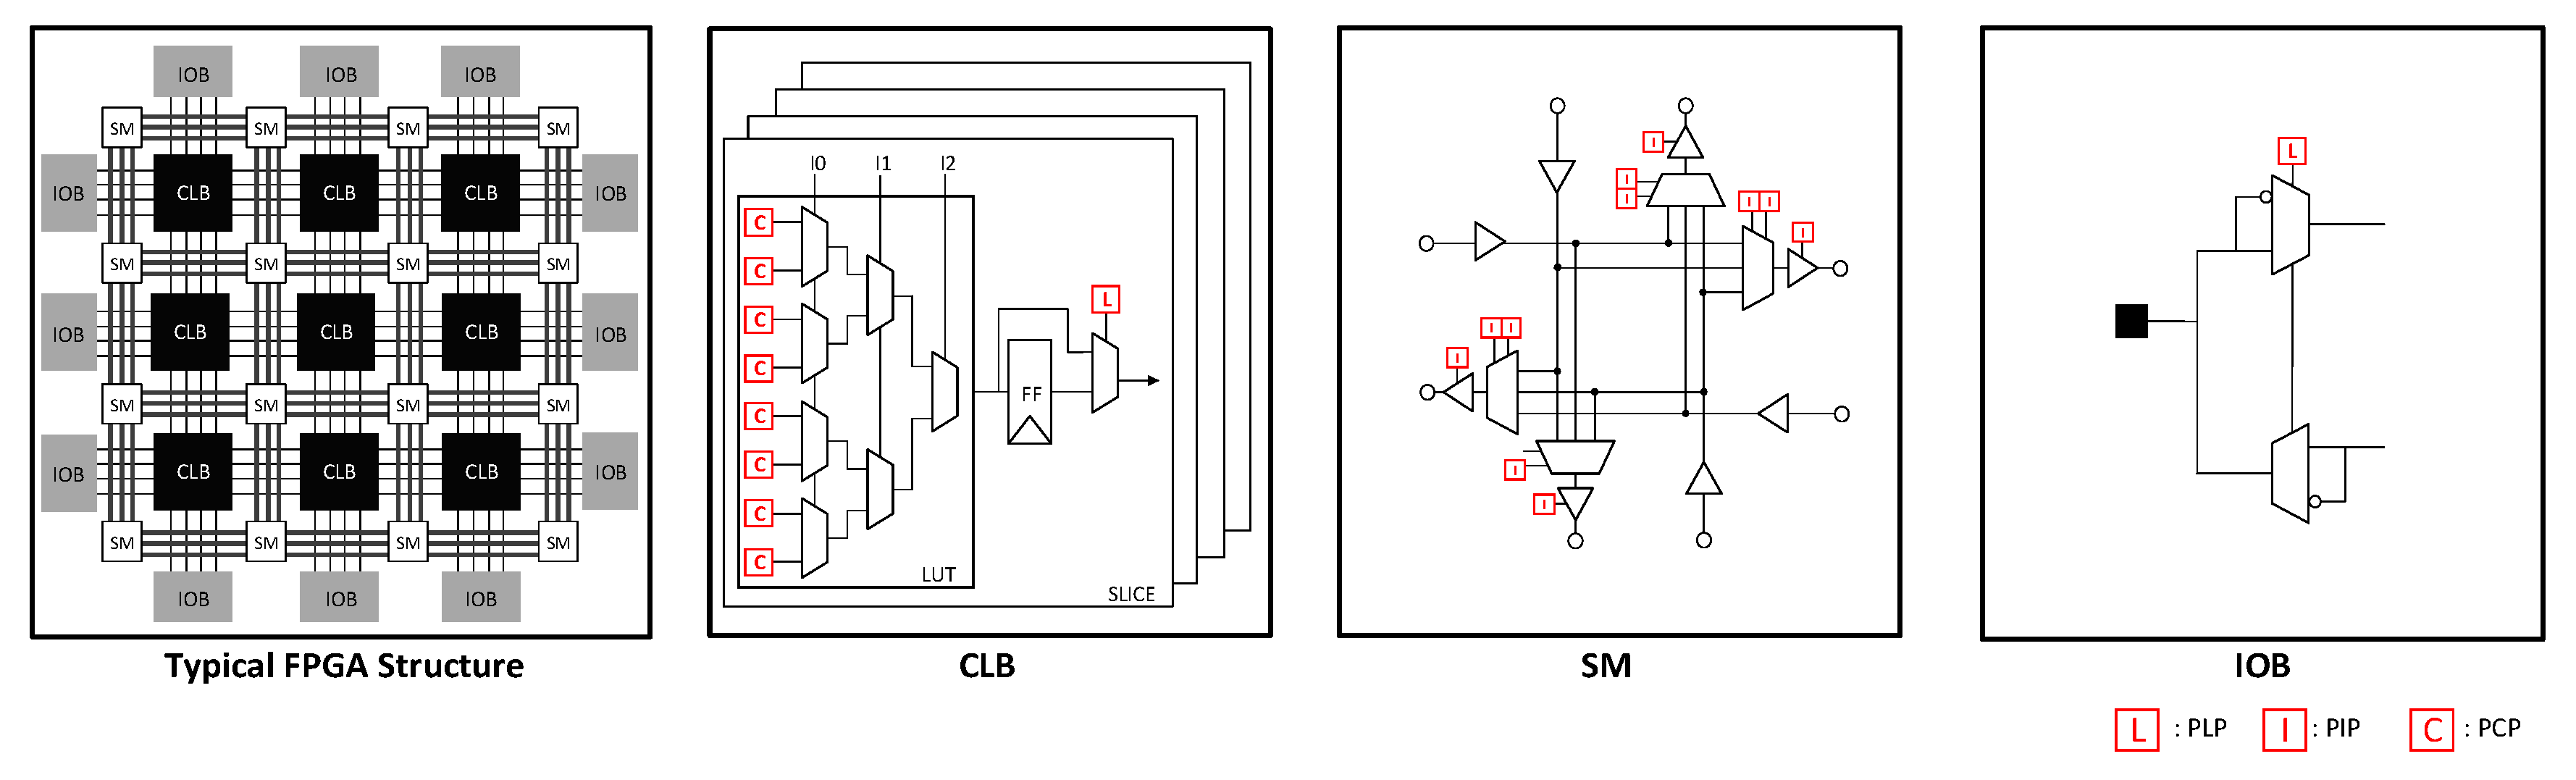
\includegraphics[width=0.9\textwidth]{fig06-fpga-tile.png}
\end{columns}
\vspace{0.5em}
\centering
\textit{FPGA = 可以被任意重新布线的 tiles 阵列。}
\end{frame}

% ============ Frame 19: Basys3与IO Planner ============
\begin{frame}{\S8 Basys3开发板与引脚分配}
\begin{columns}
\column{0.5\textwidth}
\textbf{Basys3一览：}
\begin{itemize}
  \item Xilinx Artix-7 FPGA
  \item 型号：\texttt{xc7a35t-1cpg236c}
  \item 16个用户LED、5个按键、16个拨码开关
  \item USB-UART、VGA、Pmod扩展口
\end{itemize}
\column{0.45\textwidth}
\centering
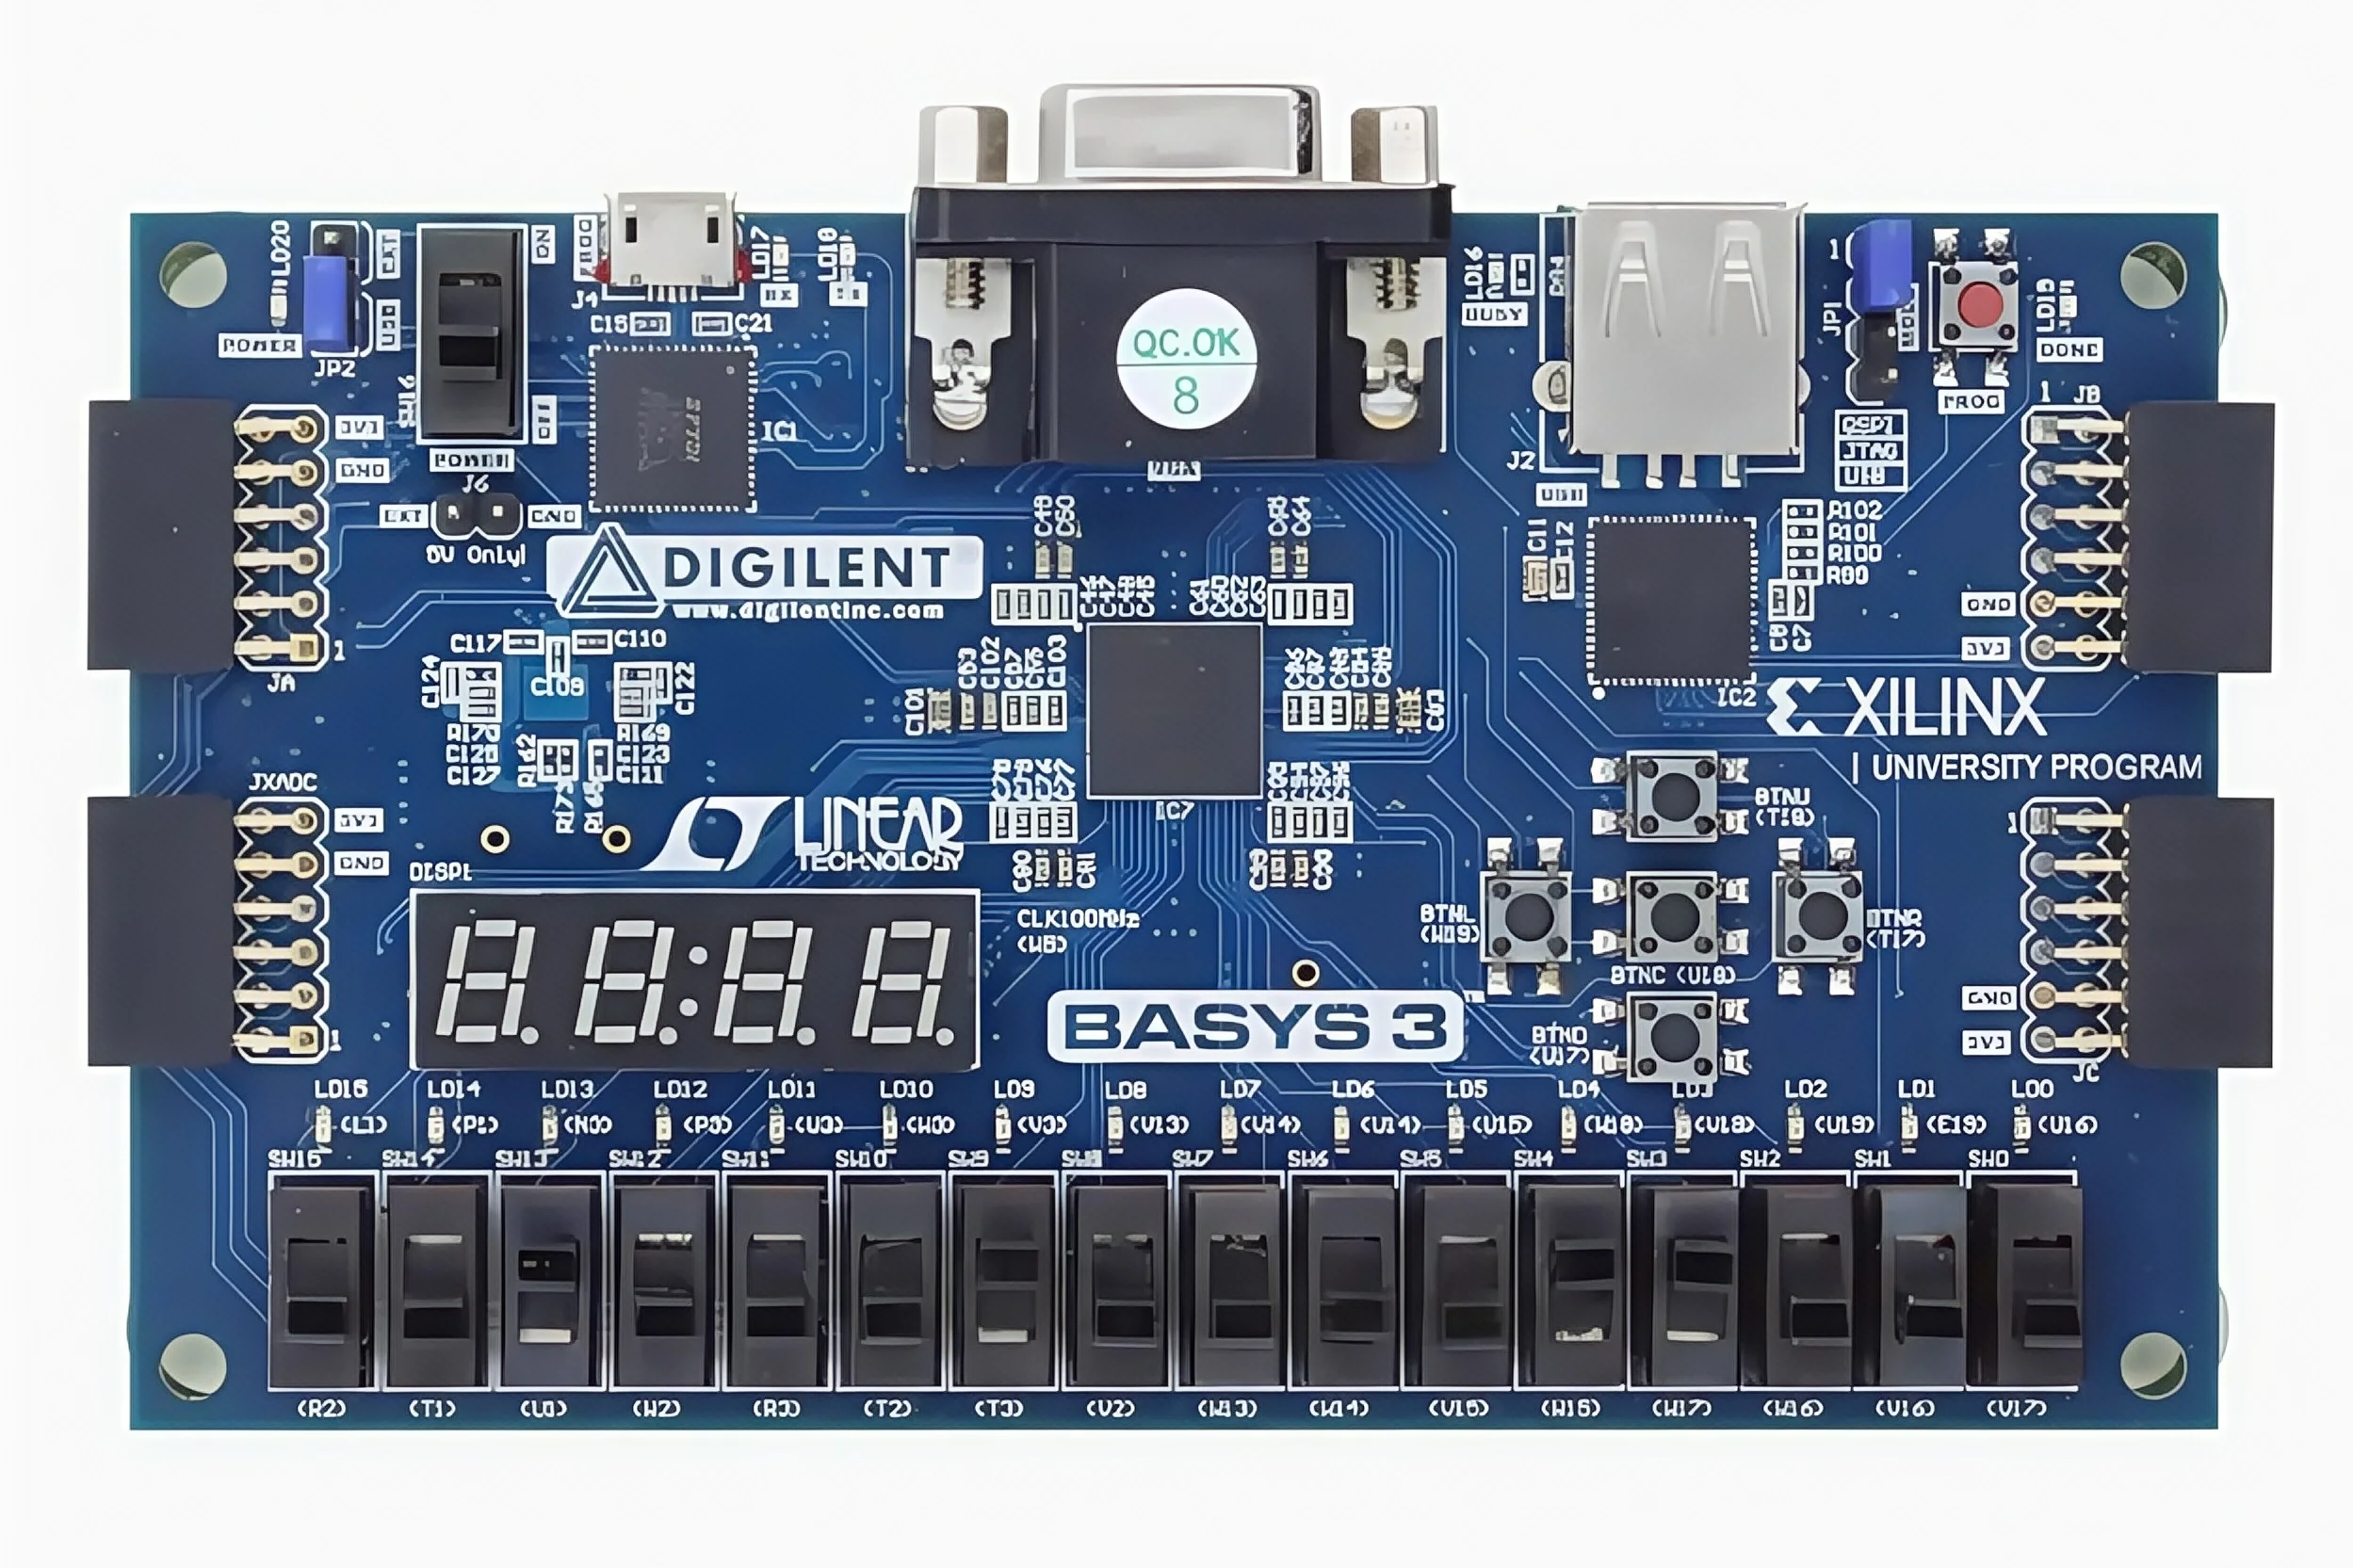
\includegraphics[width=0.85\textwidth]{fig07-basys3-photo.png}
\end{columns}
\vspace{0.5em}
\textbf{Vivado IO Planner：}把RTL端口（如 \texttt{pwm\_out}）拖拽到物理引脚（如LED0）。
\end{frame}

% ============ Frame 20: 完整闭环 ============
\begin{frame}{\S9 完整的验证闭环}
\centering
\textbf{从RTL到硬件：}
\vspace{0.3em}

\begin{tikzpicture}[node distance=1.8cm, auto]
  \node[draw, rounded corners, fill=dcMuted] (write) {写RTL};
  \node[draw, rounded corners, fill=dcMuted, right of=write] (sim) {仿真};
  \node[draw, rounded corners, fill=dcMuted, right of=sim] (wave) {看波形};
  \node[draw, rounded corners, fill=dcMuted, right of=wave] (syn) {综合};
  \node[draw, rounded corners, fill=dcMuted, right of=syn] (net) {查网表};
  \node[draw, rounded corners, fill=dcAccent!20, right of=net] (fpga) {上板};
  \draw[->, thick] (write) -- (sim);
  \draw[->, thick] (sim) -- (wave);
  \draw[->, thick] (wave) -- (syn);
  \draw[->, thick] (syn) -- (net);
  \draw[->, thick, color=dcAccent] (net) -- (fpga);
\end{tikzpicture}

\vspace{0.8em}
\begin{block}{你现在拥有了什么}
一套 \textbf{可复现、可观察的设计闭环}。\\
从第三章开始，每一个学到的概念都能在这个闭环里验证。
\end{block}
\end{frame}

% ============ Frame 21: 总结 ============
\begin{frame}{本章总结}
\begin{itemize}
  \item \textbf{Linux} 是工作界面；命令行的价值在于可复现和可脚本化。
  \item \textbf{仿真} 验证行为；\textbf{综合} 产出结构。两者都必须检查。
  \item \textbf{波形} 是主要的调试窗口——学会读时间、边沿、X/Z和占空比。
  \item \textbf{开源工具}（Icarus、GTKWave、Yosys）构成完整的学习工具链。
  \item \textbf{FPGA} 把闭环焊死在真实硬件上：写 $\rightarrow$ 仿真 $\rightarrow$ 综合 $\rightarrow$ 上板运行。
\end{itemize}
\vspace{0.5em}
\centering
\textbf{下一章：组合逻辑与布尔代数}
\end{frame}

\end{document}
